% Appendix D, Figure D.3 --- "The cubic POVM, end to end".  The layout only.
%
% Layout: card_oct_body.tex's header is binding.  Deviations from it, and only
% they, are listed here.
%
%   * the sphere column is 162pt and the table column 285pt: eight rows with
%     an effect column is the widest vertex table of the five.
%   * the key is the widest of the five (190pt): eight live cells in a
%     2 x 4 rectangle with no dead column.
%   * $\omega = +i$ is deliberately NOT printed: the chapter head states the
%     cubic circuit's Fourier convention one page earlier, and the caption
%     this card replaces never printed it either.
% All macros below are \def and therefore local to the figure environment.
\parindent=0pt \parskip=0pt
\input{../code/data/card_cube_data}
\long\def\NIS#1{\vskip #1\nointerlineskip}
\long\def\CTR#1#2{\hbox to #1{\hss #2\hss}}
\long\def\PBOX#1#2{\vtop{\hsize=#1\parindent0pt\sloppy\emergencystretch=1.5em\small #2}}
\long\def\COL#1#2{\vtop{\hsize=#1\parindent0pt\hbox{}\nointerlineskip #2}}
\long\def\FULLHEAD#1#2#3{\hbox to \hsize{\small\textbf{#1}\,#2\hfil{\footnotesize #3}}}
\def\BANDRULE{\vskip2pt\hrule height0.5pt\vskip1.5pt\nointerlineskip}
\long\def\TAB#1{{\small\renewcommand{\arraystretch}{0.88}\setlength{\tabcolsep}{3pt}#1}}
%
\vbox{\hsize\textwidth\parindent0pt
%
% --- title and the header strip: Figure 1.1's own row -----------------------
\hbox to \hsize{\large\bfseries \CTitle\hfil{\normalfont\footnotesize \CPtrStrip}}%
\NIS{5pt}%
\hbox{\CStrip}%
\BANDRULE
%
% --- band 1: the object -----------------------------------------------------
% The sphere is vertically centred against the taller eight-row effect
% table, by TeX-time arithmetic as on the octahedron card; the row's
% height is unchanged.
\FULLHEAD{1}{\CHeadA}{\CPtrA}%
\NIS{5pt}%
\setbox0=\hbox{\TAB{\CardVertexTable}}%
\setbox2=\hbox{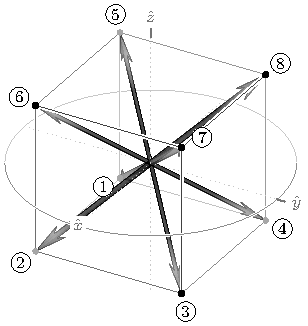
\includegraphics{figures/card_cube_sphere.pdf}}%
\dimen0=\dimexpr(\ht0+\dp0-\ht2-\dp2)/2\relax
\hbox to \hsize{%
  \COL{162pt}{\vskip\dimen0 \CTR{162pt}{\box2}}%
  \hfil
  \COL{285pt}{\hbox to 285pt{\hfil\box0}}%
}%
\NIS{4pt}%
\PBOX{\hsize}{\CIdent}%
\BANDRULE
%
% --- band 2: the machine ----------------------------------------------------
\FULLHEAD{2}{\CHeadB}{\CPtrB}%
\NIS{5pt}%
\hbox to \hsize{%
  \COL{268pt}{\hbox to 268pt{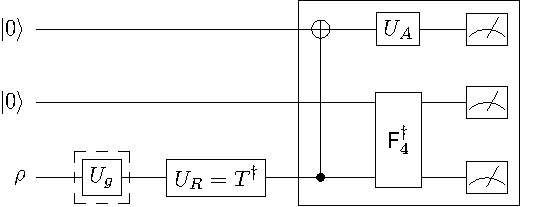
\includegraphics{figures/card_dec_cube.pdf}\hss}}%
  \hfil
  \COL{179pt}{\small\CardSide}%
}%
\NIS{5pt}%
\PBOX{\hsize}{\CParams}%
\BANDRULE
%
% --- band 3: the readout ----------------------------------------------------
\FULLHEAD{3}{\CHeadC}{\CPtrC}%
\NIS{5pt}%
\hbox to \hsize{%
  \COL{190pt}{\TAB{\CardKey}}%
  \hfil
  \COL{254pt}{\PBOX{254pt}{\CKappa}}%
}%
\BANDRULE
%
% --- band 4: the alternative ------------------------------------------------
\FULLHEAD{4}{\CHeadD}{\CPtrD}%
\NIS{5pt}%
\PBOX{\hsize}{\CRays}%
\NIS{2pt}%
\PBOX{\hsize}{\CCoin}%
}%
